%***********************************************************************************************
% Memo Micro SETTINGS
%***********************************************************************************************
\newcommand{\WorkWeek}{1252} % Current Work Week (later we should write a script to decide this)
\newcommand{\BossName}{Arden Chang} % Boss’s Name
\newcommand{\BossInitials}{ARDN} % Boss’s Initials
\newcommand{\Author}{Qiling Bo} % Author’s Name
\newcommand{\AuthorInitials}{QIBO} % Author’s Cypress Initials
\newcommand{\MemoNumber}{077} % Memo number
\newcommand{\Subject}{TEST SOFTWARE SOURCE CODE VERSION CONTROL INTRODUCTION} % Subject of the memo
\newcommand{\Category}{Trackpad, Version Control} % Keywords for the memo
\newcommand{\Distribution}{PZHO, MZFA, WEIQ, ARDN, RQB} % Distribution list for the memo

%***********************************************************************************************
% Rules
%***********************************************************************************************

% The following characters play a special role in LaTeX:
%
%        # $ % & ~ _ ^ \ { }
%
%If you simply want the character to be printed just as any other letter, 
%include a \ in front of the character. For example, \$ will produce $ in your output. 

%***********************************************************************************************
% Document SETTINGS
%***********************************************************************************************
\documentclass{article}

\usepackage{amsmath}
\usepackage{amsfonts}
\usepackage{amssymb}
\usepackage{fullpage}
\usepackage{graphicx} % Required to insert images
\usepackage{alltt}
\usepackage{color}
\usepackage{hyperref} % For hyper link
\usepackage{float}
\setlength{\headheight}{11pt}
\usepackage{subfigure}


%***********************************************************************************************
% Make Title
%***********************************************************************************************
\renewcommand{\maketitle}
{
%   \\
%   \vspace{-1.25 in}
    \begin{center}
    
\includegraphics[width=2.5in]{./template/CY.jpg}\\
    \vspace{5 mm}
    \large
    {
    \textbf{CYPRESS SEMICONDUCTOR CORPORATION}\\
    \textbf{Internal Correspondence}\\
    }
    \vspace{1 mm}
    \hspace{0.5 in}
    \begin{tabular}{rl}
    \bf Date: & \today\ \hspace{2 in}\textbf{WW:\ }\WorkWeek\\
    \bf To: & \BossName\ (\BossInitials)\\
    \bf Author: & \Author\ (\AuthorInitials)\\
    \bf Author File \#: & \AuthorInitials\#\MemoNumber\\
    \bf Subject: & \Subject\\
    \bf Category: & \Category\\
    \bf Distribution: & \Distribution\\
    \end{tabular}
    \vspace{3 mm}\\
    \hrule
    \end{center}
    
    \thispagestyle{firstpage}
    \pagestyle{normalpage}
}


%***********************************************************************************************
% Font
%***********************************************************************************************
% - Helvetica
%\usepackage[scaled]{helvet}
%\renewcommand*\familydefault{\sfdefault} %% Only if the base font of the document is to be sans serif
%\usepackage[T1]{fontenc}

% - Times
%\usepackage{fontspec}
\usepackage{mathptmx}
\usepackage[T1]{fontenc}
%\setmonofont{DejaVu Sans Mono}

%***********************************************************************************************
% Custom Color
%***********************************************************************************************
\definecolor{gray}{rgb}{0.9,0.9,0.9} %for source code display
\definecolor{dkgreen}{rgb}{0.1333,0.5451,0.1333}

%***********************************************************************************************
% Header and Footer
%***********************************************************************************************
\usepackage{fancyhdr} % Required for custom headers

\fancypagestyle{firstpage}{%
  
  \fancyhf{} % clear all header and footer fields
  \fancyfoot[L]{\small{\bf{\thepage}}}
  \fancyfoot[R]{\Author\ (\AuthorInitials)}
  \renewcommand{\headrulewidth}{0.0pt}%
}

%\pagestyle{fancy}
\fancypagestyle{normalpage}{%
    \fancyhf{} % clear all header and footer fields
    \fancyhead[C]{\small{\Subject}}
    \fancyfoot[L]{\small{\bf{\thepage}}}
    \fancyfoot[R]{\Author\ (\AuthorInitials)}
    
    \renewcommand{\headrulewidth}{0.4pt}
    \renewcommand{\footrulewidth}{0.4pt}
    
    \renewcommand{\headsep}{25pt}
}

%\AtBeginDocument{
%    \thispagestyle{firstpage}
%    }

%***********************************************************************************************
% Source code display Setting
%***********************************************************************************************
\usepackage{listings}
\usepackage{courier}

\lstloadlanguages{Python}
\lstset{
     language=Python,
     keywords={from,import,break,case,catch,continue,else,elseif,end,for,def,global,if,otherwise,persistent,return,switch,try,not,while,True,False,in},
     basicstyle=\footnotesize\ttfamily,
     tabsize=2,                   
     extendedchars=true,         
     breaklines=true,            
     keywordstyle=\color{blue},
     frame=none,                    % tb-for top and bottom, single-for around         
     stringstyle=\color{red}\ttfamily, 
     commentstyle=\color{dkgreen},
     backgroundcolor=\color{gray},
     showspaces=false,           
     showtabs=false,             
     xleftmargin=17pt,
     framexleftmargin=17pt,
     framexrightmargin=5pt,
     framexbottommargin=4pt,     
     showstringspaces=false 
}
% Creates a new command to include a C source, the first parameter is the filename of the script (without .c), the second parameter is the caption
\newcommand{\PythonSource}[2]{
\begin{itemize}
\item[]\lstinputlisting[caption=#2,label=#1]{#1.py}
\end{itemize}
}

%***********************************************************************************************
% Figure 
%***********************************************************************************************
%\MySubFigureTwo{./data/IDAC_hist.pdf}{./data/IDAC_hist_2.pdf}{Dynamic}{HuaXin}{0.2in}{IDAC Histogram}{fig1}{0.5}
\newcommand{\MySubFigureTwo}[8]
{
    \vspace{#5}
    \begin{figure}[H]
    \centering
    \subfigure[#3]
    {
        \includegraphics[scale=#8]{#1}
        \label{fig:a#7}
    }
    \subfigure[#4]
    {
        \includegraphics[scale=#8]{#2}
        \label{fig:b#7}
    }
    \caption[#6]{#6}
    \label{fig:#7}
    \end{figure}
}


%***********************************************************************************************
% Document Begin
%***********************************************************************************************
\begin{document}

\maketitle

%------------------------------------ %
%								     %
%--------START YOUR MEMO HERE-------- %
%									 %
%------------------------------------ %

\section{INTRODUCTION}
This memo introduces the basic functions of subversion(SVN). \\
The definition of subversion on wikipedia:
SVN is a software versioning and revision control system distributed under an open source license. Developers use Subversion to maintain current and historical versions of files such as source code, web pages, and documentation.

\section{SVN BASIC COMMANDS}

\begin{itemize}
\item
	\textbf{Install}\\
	Use the "apt-get" commmand to install the svn on Ubuntu, or download TortoiseSVN for Windows OS.
	\begin{lstlisting}
	sudo apt-get install subversion	
	\end{lstlisting}

\item
	\textbf{Check Out}\\
	Use "svn checkout" to checkout a project on the repository. This example will create a "Macross" folder for the project Macross, and check out the trunk of Macross project from repository to native working copy.
	\begin{lstlisting}
	svn checkout http://172.23.6.12/repos/BMOChina/Public/Source/Macross/trunk Macross
	\end{lstlisting}

\item
	\textbf{Check Status}\\
	Use svn status to check the status of native working copy. The un-versioned files are marked with a quesiton mark. The modified files are marked with a "M".
	\begin{lstlisting}
	svn status
	\end{lstlisting}

\item
	\textbf{Add}\\
	Add items into version control. With add * will all un-versioned to version control.
	\begin{lstlisting}
	svn add *
	\end{lstlisting}	

\item
	\textbf{Commit}\\
	After added the items, we need commit the changes to the repository.
	\begin{lstlisting}
	svn commit -m "change something."
	\end{lstlisting}

\item
	\textbf{Update}\\
	Synchronize the local working copy items to the repository.
	\begin{lstlisting}
	svn update
	\end{lstlisting}

\end{itemize}

\section{SVN TRUNK BRANCHES \& TAGS}
\begin{itemize}
\item
	Directory for trunk, branches and tags. See Figure 1. \\
	The explanation from StackOverFlow, http://stackoverflow.com/questions/16142/
	\begin{itemize}
	\item[-]
    \textbf{Trunk} would be the main body of development, originating from the start of the project until the present.
	\item[-]
    \textbf{Branch} will be a copy of code derived from a certain point in the trunk that is used for applying major changes to the code while preserving the integrity of the code in the trunk. If the major changes work according to plan, they are usually merged back into the trunk.
	\item[-]
    \textbf{Tag} will be a point in time on the trunk or a branch that you wish to preserve. The two main reasons for preservation would be that either this is a major release of the software, whether alpha, beta, RC or RTM, or this is the most stable point of the software before major revisions on the trunk were applied.
	\end{itemize}
	
\begin{figure}[h]
\label{fig:fig_svn}
\begin{center}
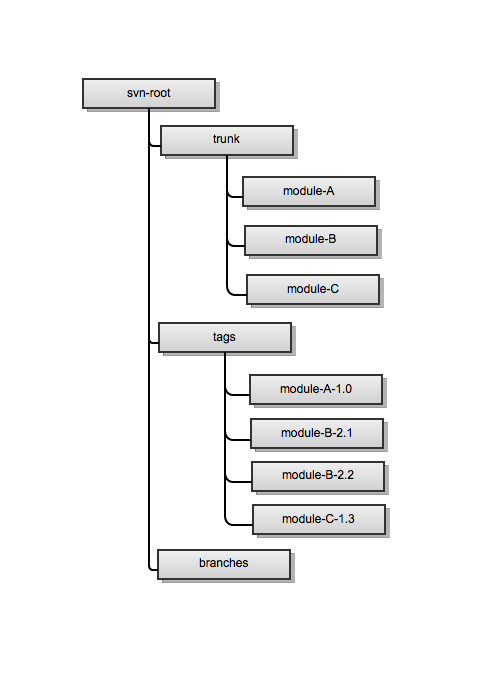
\includegraphics[scale=0.5]{spice-svn.png}
\caption{The SVN project directory structure}
\end{center}
\end{figure}	
	
\item
	Create a branch.\\
	For example, create a branch named "qibo-branch" for Macross project.
	\begin{lstlisting}
	svn cp http://172.23.6.12/repos/BMOChina/Public/Source/Macross/trunk \
	http://172.23.6.12/repos/BMOChina/Public/Source/Macross/branches/qibo-branch
	\end{lstlisting}	
\textit{Note that a backslash ($\setminus$) means that the command continues onto the next line.}	
\item
	Switch to a working copy from that branch. \\ 
	Assuming that we have already check out the trunk version. We need to switch to the branch we created.
	\begin{lstlisting}
	svn switch http://172.23.6.12/repos/BMOChina/Public/Source/Macross/branches/qibo-branch
	\end{lstlisting}	
	Every time you switch the branch, you will exactly check out that branch, and change the working copy.
\item
	Check which branch the local copy is.
	\begin{lstlisting}
	svn info | grep "URL"
	\end{lstlisting}	
\textit{Note that we used a regular express "URL" after the grep, to display the information has "URL" only.}
\item
	Now you can make some changes to current working copy and commit the changes to current branch.
	\begin{lstlisting}
	svn commit -m "some changes on branch"
	\end{lstlisting}	
\item
	Delete a branch. \\ 
	If we don't need the branch qibo-branch, we can delete it remotely.
	\begin{lstlisting}
	svn del http://172.23.6.12/repos/BMOChina/Public/Source/Macross/branches/qibo-branch
	\end{lstlisting}
\end{itemize}

\section{MERGE THE CODE}
Suppose we have 2 developers A and B working on their own branches, A is working on module A and B is working on module B, and at last, we want to have a trunk with both module A and module B working together.\\
There are some rules to make things easier.
\begin{itemize}
\item[-] Change the software structure on the trunk. Avoid to change it on the branches.
\item[-] Once get a branch copy, don't delete the folders or files from the original copy, to avoid the conflicts.
\item[-] For some common usage files, try to add some temp files to test the function or interface.
\item[-] Try to merge the code from trunk to branch and from branch to trunk, avoid to merge the code from branch to another branch.
\item[-] Before merge the code, better to release a tag first.
\end{itemize}
\textit{Note that these rules are not necessary, but can help us to merge the code successfully.}


\subsection{From branch to trunk}
Suppose now we are working on a branch, and we made some changes and this branch works great. Now we need to merge the code to the trunk, so other team member can get the copy, and we can follow the next a few steps.

\begin{itemize}
\item 
	Make sure the working copy are synchronized with the branch, update and commit the changes.
	\begin{lstlisting}
	svn update 
	svn commit -m "last changes before merge"
	\end{lstlisting}

\item 
	Check the last merge revision of your branch, and check the head version of the trunk.
	\begin{lstlisting}
	//get LAST_MERGED_REVISION
	svn log --limit 500 | grep -B 3 qibo-branch
	
	//get HEAD_REVISION 											  
	svn info http://172.23.6.12/repos/BMOChina/Public/Source/Macross/trunk | grep Revision  
	\end{lstlisting}

\item
	Switch to the trunk.
	\begin{lstlisting}
	//switch to the trunk
	svn switch http://172.23.6.12/repos/BMOChina/Public/Source/Macross/trunk	
	\end{lstlisting}

\item
	Merge the code to the updated branch. Very important here to note that, the merged result only affect the local working copy.
	\begin{lstlisting}
	svn merge -r HEAD_REVISION:LAST_MERGED_REVISION \
	  http://172.23.6.12/repos/BMOChina/Public/Source/Macross/branches/qibo-branch
	\end{lstlisting}

\item
	If any conflicts or errors, we can revert back or solve the conflicts.
	\begin{lstlisting}
	//revert	
	svn revert -R *
	
	//check conflicts
	svn status | egrep '^C|^.C'
	\end{lstlisting}
	\textit{Note that regular express '\^{}C $\vert$ \^{}.C' means any string starts with C or .C}

\item
	Commit the merge result to trunk.
	\begin{lstlisting}
	svn commit -m "merge successful message"
	\end{lstlisting}
\end{itemize}

\begin{figure}[h]
\label{fig:fig_merge}
\begin{center}
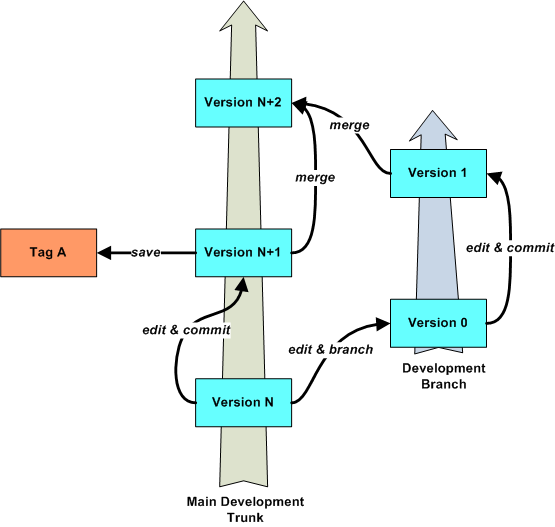
\includegraphics[scale=0.5]{svn_merge.png}
\caption{The general process of code merge}
\end{center}
\end{figure}	


\subsection{From trunk to branch}
Suppose now we are working on a branch, and some one update an amazing function on the trunk, and we want to have a try on our own branch, and we can follow the next a few steps.

\begin{itemize}
\item
	Make sure the working copy are synchronized with the branch, update and commit the changes.
	\begin{lstlisting}
	svn update 
	svn commit -m "last changes before merge"
	\end{lstlisting}

\item
	Check the last merge revision of your branch, and check the head version of the trunk.
	\begin{lstlisting}
	//get LAST_MERGED_REVISION
	svn log --limit 500 | grep -B 3 qibo-branch
	
	//get HEAD_REVISION 											  
	svn info http://172.23.6.12/repos/BMOChina/Public/Source/Macross/trunk | grep Revision  
	\end{lstlisting}

\item
	Merge the code to the trunk. Very important here to note that, the merged result only affect the local working copy.
	\begin{lstlisting}
	svn merge -r HEAD_REVISION:LAST_MERGED_REVISION \
	  http://172.23.6.12/repos/BMOChina/Public/Source/Macross/trunk
	\end{lstlisting}

\item
	If any conflicts or errors, we can revert back or solve the conflicts.
	\begin{lstlisting}
	//revert	
	svn revert -R *
	
	//check conflicts
	svn status | egrep '^C|^.C'
	\end{lstlisting}

\item
	Commit the merge result to the branch.
	\begin{lstlisting}
	svn commit -m "merge successful message"
	\end{lstlisting}
\end{itemize}

%------------------------------------ %
%								      %
%--------END OF YOUR MEMO HERE------- %
%									  %
%------------------------------------ %



\end{document}
%***********************************************************************************************
% Document End
%***********************************************************************************************


